\documentclass[../uilmath.tex]{subfiles}
\graphicspath{{\subfix{../figures/}}}
\begin{document}
\chapter{Pre-Calculus}
\section*{Problems}
\begin{enumerate}[label=\bfseries\arabic*.]
    \item %% Problem 1
    The graph of $x^2+y^2-4x+12y+30=0$ is a circle with a diameter of: 

    \item %% Problem 2
    Let $\tan A = \frac{7}{24}$, where $A$ is in QIII. Find $\cos A$.

    \item %% Problem 3
    An equivalent expression for $(\sin x + \cos x)^2+(\sin x - \cos x)^2$ is:

    \item %% Problem 4
    The graph of $x^2+y^2+10x-12y-20=0$ is a circle with a radius of:

    \item %% Problem 5
    A cliff near a lake is 125 feet high. The angle of depression of a canoe from the top of the cliff is 30$\degree$. How far is the canoe from the base of the cliff? (nearest foot).

    \item %% Problem 6
    Simplify: $\sin\theta \tan\theta + \cos\theta$

    \item %% Problem 7
    Use the angle of rotation, $\theta$ (nearest degree), where 0$\degree<\theta<90\degree$, to transform the conic $xy=1$ into an equation that is in standard position and does not contain an $xy$ term. The transformed equation is:

    \item %% Problem 8
    The focus of the parabola below has coordinates $(a,b)$. $a+b=\blank$.
    \begin{center}
        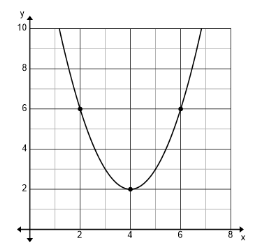
\includegraphics[width=0.3\textwidth]{2021SAC9.PNG}
    \end{center}

    \item %% Problem 9
    Find the eccentricity of the ellipse. $9x^2+16y^2-36x+96y+36=0$. (nearest hundredth)

    \item %% Problem 10
    Simplify: $4\csc(2x)\cos(x)$

    \item %% Problem 11
    Polonium 221 has a half-life of 130 seconds. How long will it take a sample with a mass of 1.80 g to decay to a mass of 1.20 g? (nearest tenth)

    \item %% Problem 12
    Assume the number of hours of daylight varies sinusoidally at the Clydehurst Christian Ranch in Montana. The longest day of the year has 15 hr 30 min of daylight and the 
    shortest day has 8 hr 30 min of daylight. How many days during the year have at least 13 hours of daylight?

    \item %% Problem 13
    The Holiday Inn is across the street from the Hilton. The hotels are 120 feet apart. Joe looks out the window of his room 
    at the Holiday Inn and notices that the angle of depression to the base of the Hilton is $36\degree$ and the angle of elevation 
    to the top of the Hilton is $44\degree$. How tall is the Hilton? (nearest foot)

    \item %% Problem 14
    The graph of $r=3-3\sin\theta$ is a \blank.

    \item %% Problem 15
    The graph of the parametric equations $x=2+3\cos\theta$ and $y=1+2\sin\theta$ is an ellipse with vertices 
    $(a,b)$ and $(c,b)$. $a+c=\blank$.

    \item %% Problem 16
    If $\frac{12i+8i^4+12i^3}{\sqrt{-100}+10i+6i^4}$ simplifies to $\frac{a}{b}+\frac{c}{b}i$, then $a+b+c=\blank$.

    \item %% Problem 17
    If $f(x)=\sec(2x)$ and $h(x)=\csc(3x)$. $f\left(\frac{5\pi}{8}\right)+h\left(\frac{11\pi}{18}\right)=\blank$. (nearest tenth)

    \item %% Problem 18
    Each of the wheels on Russell's jumbo wheel swamp buggy has a 4 ft diameter. When he is traveling 42 mph, what 
    is the angular velocity of the wheels in revolutions per minute? (nearest whole number)

    \item %% Problem 19
    The vertex of the parabola $y=-4x^2+6x-8$ is the point $(a,b)$. $a+b=\blank$. (nearest hundredth)

    \item %% Problem 20
    Multiply $(6\cis(60\degree))(-4\cis(-150\degree))$ and express the result in rectangular form.

    \item %% Problem 21
    Sarah released 36 bunnies into the woods near her house. Six months later the population had increased to 
    100 bunnies. Assume the bunny population is increasing exponentially and calculate the expected bunny population 21 months after the original release of 36 bunnies.

    \item %% Problem 22
    Devin drops a ball from a height of 24 feet. On each bounce, the ball rebounds three-fourths of the distance it fell. How far does the ball rebound on the tenth bounce? (nearest inch)

    \item %% Problem 23
    Consider $f(x)=x^3+bx^2+cx+d=0$. Two of the zeroes are $5$ and $2i$. $\mid b+c+d \mid=\blank$.

    \item %% Problem 24
    The vertices of the hyperbola $16y^2-9x^2-96y-72x-144=0$ are $(a,b)$ and $(a,c)$. $b+c=\blank$.

    \item %% Problem 25
    Consider a parabola with vertex $\left(\frac{3}{2},\frac{1}{4}\right)$. If the point 
    $(-2,4)$ lies on the graph of the parabola, which of the following points also lies on the graph of the parabola? The graph is concave up.

    $\textbf{(A) } (2,-2) \qquad \textbf{(B) } (3,0) \qquad \textbf{(C) } (4,2) \qquad \textbf{(D) } (5,4) \qquad \textbf{(E) } (6,6)$

    \item %% Problem 26
    Find the angle between the line $3x-y=6$ and the line $4x+5y=9$. (nearest tenth)

    \item %% Problem 27
    The graph of the polar equation $r=3-3\cos(\theta)$ is a $\blank$.

    \item %% Problem 28
    The graph of the parametric equations $x=13\cos(\theta)$ and $y=5\sin(\theta)$ is an ellipse with a foci $(a,b)$ and $(c,b)$. $\mid a-c \mid = \blank$.

    \item %% Problem 29
    Consider the sphere $x^2+y^2+z^2+4x-6y+2x-11=0$. Find the volume of the sphere. (nearest tenth)

    \item %% Problem 30
    The unit vector orthogonal to both $u=2i-3j+4k$ and $v=-2i+5j-7k$ is the vector 
    $\frac{a}{\sqrt{53}}i+\frac{b}{\sqrt{53}}j+\frac{c}{\sqrt{53}}k$. $a+b+c=\blank$.

    \item %% Problem 31
    Which of the following is not one of the fourth roots of $16(\cos 120\degree + i\sin 120\degree)$?

    $\textbf{(A) } -\sqrt{3}-i \qquad \textbf{(B) } \sqrt{3}+i \qquad \textbf{(C) } 1-\sqrt{3}i \qquad \textbf{(D) } -\sqrt{3}+i \qquad \textbf{(E) } -1+\sqrt{3}i$

    \item %% Problem 32
    Suppose Calvin has 112 mg of bismuth-214 at 12:15 PM. His sample undergoes radioactive decay and is 
    reduced to 74.562 $\mu$g at 3:45 PM the same day. Find the half-life os bismuth-214. (nearest tenth)


    For problems 33 and 34, consider the parabola with equation $9y=2x^2-8x-46$.
    \item %% Problem 33
    The vertex of the graph of the parabola is the point $P(a,b)$. $a+b=\blank$.

    \item %% Problem 34
    The equation of the directrix of the graph of the parabola is $y=\blank$.

    \item %% Problem 35
    Consider the ellipse with equation $16x^2+9y^2+64x-54y+1=0$. The vertices of the graph of the ellipse are 
    $(a,b)$ and $(a,c)$. $a+b+c=\blank$.

    \item %% Problem 36
    Consider the hyperbola with equation $9x^2-4y^2-108x-16y+272=0$. The eccentricity 
    of the hyperbola is \blank. (nearest tenth)

    \item %% Problem 37
    A stick in the ground is 4 ft 8 in tall and it casts a shadow that is 6 ft 2 in long. At the same time, 
    the Newcastle State Bank casts a shadow that is 90 ft long. How tall is the bank? (nearest foot)

    \item %% Problem 38
    A guy wire runs from the groudn to the top of a 42-foot pole. The angle formed between the wire and the pole is 44$\degree$. How far 
    from the base of the pole is the wire attached to the ground? (nearest tenth)

    \item %% Problem 39
    Given $\vec{v}=\langle 1,2,3 \rangle$ and $\vec{w}=\langle 4,5,6 \rangle$. The unit vector in the direction $2\vec{v}+3\vec{w}$ is the 
    vector $\left\langle \frac{a}{d},\frac{b}{d},\frac{c}{d}\right\rangle$ where $d=\blank$. (nearest hundredth)

    \item %% Problem 40
    Consider the circle $x^2+y^2+14x-6y+9=0$. The area of the circle is $\blank$. (nearest tenth)

    \item %% Problem 41
    If a 56-ft-tall tree produces a shadow that is 12 ft long, how long will the shadow be for a person that is 5 ft tall? (nearest hundredth)

    \item %% Problem 42
    The graph of the circle $x^2+y^2=49$ and the graph of the line $y=0.6x+5$ intersect at points $A$ and $B$. $AB=\blank$. (nearest tenth)

    \item %% Problem 43
    The graph of $y=3\tan(.25x)$ has a vertical asymptote at $x=\blank$.

    \item %% Problem 44
    The relation $\{(0,0), (2,2), (2,-2), (6,8), (6,-8)\}$ is:

    \item %% Problem 45
    A hawk is perched at the edge of a roof of the Denver City State Bank. The hawk spots a mouse on the ground below. The angle of depression from the hawk to the 
    mouse is $22\degree$. The mouse is located 154 feet from the base of the bank. How tall is the Denver City State Bank? (nearest foot)

    \item %% Problem 46
    On March 1st of 2015, Piyush's father placed \$75,000 into an account for Piyush that earns interest at a rate of 6.75\% compounded 
    quarterly. Piyush plans to withdraw all of the money in the account on March 1st of 2025 and use it toward the purchase of a new BMW X7 From 
    Grapevine BMW. If the total cost including tax, title and license is \$146,875.19 how much money will Piyush have to come up with? (nearest dollar)

    \item %% Problem 47
    Consider the circle $x^2+y^2+ax+by+c=0$. The center of the circle is at the point $(2,5)$ and the diameter is 14. $a+b+c=\blank$.

    \item %% Problem 48
    A population of Fire Ants is increasing exponentially in Hale County. Phoenix introduced a population of 150 ants at $t=0$. 
    At $t=60$ days, the population reached 1800 ants. The population should reach 212,000 ants at $t=\blank$ days. (nearest whole number)

    \item %% Problem 49
    Austin leaves the Lubbock airport at 2:00 PM and flies on a bearing of $60\degree$ at a speed of 180 mph. At 2:30 PM, Zhikai 
    leaves the Lubbock airport and flies on a bearing of 195$\degree$ at a speed of 160 mph. How far apart are they at 4:00 PM? (nearest mile)

    \item %% Problem 50
    Consider an ellipse centered at $(4,3)$ with a vertex at $(-2,3)$. The point $(4,7)$ lies on the ellipse.
    The area of the ellipse is \blank. (nearest tenth)

    \item %% Problem 51
    Consider the curve represented by the parametric equations $x=6\cos(\theta)$ and $y=4\sin(\theta)$. The 
    distance between the foci is \blank. (nearest tenth)

    \item %% Problem 52
    Given: $\vec{v}=\langle 1,2,3 \rangle$ and $\vec{w}=\langle 4,6,8\rangle$. The unit vector in the direction of 
    $2\vec{v}+3\vec{w}$ is the vector $\left\langle \frac{a}{d}, \frac{b}{d}, \frac{c}{d}\right\rangle$ where $d=\blank$. (nearest hundredth)

    \item %% Problem 53
    Consider the hyperbola with equation $4y^2-9x^2+16y+108x-344=0$. The eccentricity of the hyperbola is $\blank$. (nearest tenth)

    \item %% Problem 54
    Geometry class ends when the bell rings at 8:50. Bo Ring looks at the circular clock and sees that the time is 8:30. How much bigger is the angle formed 
    by the hands at 8:30 then the angle formed when the bell rings?

    \item %% Problem 55
    The \blank of a hyperbola is equal to the ratio of the distance between the center and a focus 
    to the distance between the center and the corresponding vertex.

    \item %% Problem 56
    The highest average monthly temperature for Miller's View is 78.5$\degree$ F and occurs in July. The lowest average 
    monthly temperature occurs in January and is 43.5$\degree$ F. The average monthly temperature 
    of Miller's View varies sinusoidally with the month. What would be the predicted average temperature for May? (nearest tenth)

    \item %% Problem 57
    If the $\cos A = .96$ and $A$ is in QIV, then $\cot A$ is: 

    \item %% Problem 58
    Which of the following is NOT a solution for $\cos\theta + 1 =\cos^2\theta$?

    $\textbf{(A) } \frac{8\pi}{3} \qquad \textbf{(B) } \frac{4\pi}{3} \qquad \textbf{(C) } -\frac{2\pi}{3} \qquad \textbf{(D) } -\pi \qquad \textbf{(E) } -4\pi$

    \item %% Problem 59
    $(1-i)^7$ equals:

    \item %% Problem 60
    A ramp rises $\frac{1}{4}$ inch for every foot of run. Find the angle the end of the ramp 
    makes with the ground if the ramp is 12 feet long. (nearest tenth of a degree)

    \item %% Problem 61
    If $3\sin\theta + 4\cos\theta = 5$ then $\tan\theta$ is: 

    \item %% Problem 62
    The directrix of the parabola $y=-(x^2+2x+5)$ is $y=\blank$.

    \item %% Problem 63
    How many points of intersections do the graphs of $r=3\cos\theta$ and $\theta=-\frac{\pi}{2}$ have?
    
    \item %% Problem 64
    Diamond Jim deposited some money in a savings account 30 months ago at a rate of 2.5\% compounded monthly.
    His current balance is \$553.50. How much was his original deposit?

    \item %% Problem 65
    The equation $y=\blank$ will produce this graph.
    \begin{center}
        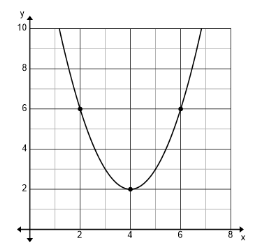
\includegraphics[width=0.4\textwidth]{2021SAC9.PNG}
    \end{center}

    \item %% Problem 66
    Determine the type of conic section this equation $x^2+2xy+y^2-6x-6y+9=0$ will produce.

    \item %% Problem 67
    Determine the period of the function $y=3-2\cos\left(\frac{x}{4}+\pi\right)$

    \item %% Problem 68
    How many points of intersections are there for the curves $r=2\sin\theta$ and $r=2\sin\theta$?

    \item %% Problem 69
    The directrix for the parabola $-8y=x^2$ is $y=\blank$.

    \item %% Problem 70
    Let $\frac{6x^2}{5}-\frac{3xy}{2}+\frac{19y^2}{5}-4=0$. What is the angle of rotation from it's parent function? (nearest degree)

    \item %% Problem 71
    Vector $v=(8,6,-2)$ and vector $u=(-4,x,1)$. Find $x$ if the dot product of vectors $u$ and $v$ is 2.

    \item %% Problem 72
    A porch is 3 feet high. A ramp is built to reach from the porch to the ground with an angle of elevation of $15\degree$.
    How far from the base of the porch does the ramp touch the ground? (nearest inch)

    \item %% Problem 73
    Two circles, $(x-2)^2+(y-5)^2=25$ and $(x-6)^2+(y-13)^2=65$, intersect at two points. Find the equation of the line passing through the two points of intersection.

    \item %% Problem 74
    Find the unit vector in the same direction as $(8,15)$.

    \item %% Problem 75
    Find the value of $\sin(\arcsin\frac{1}{2}-\arccos \frac{1}{2})$.

    \item %% Problem 76
    A scout troop leaves their vehicles and travels on a hike of 2 km on a bearing of $45\degree$ to Camp Fife for a swim. Then they travel 3 km on a bearing of $135\degree$ to the scout lodge for lunch. What is the 
    least distance they will have to hike to return to their vehicles? (nearest tenth)

    \item %% Problem 77
    The equation $y=\blank$ will produce this graph.
    \begin{center}
        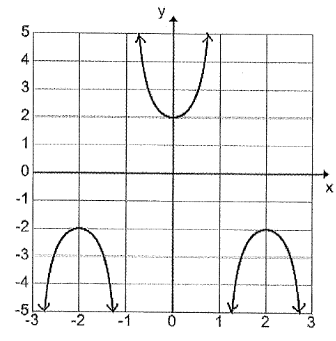
\includegraphics[width=0.4\textwidth]{2008B57.PNG}
    \end{center}

    \item %% Problem 78
    A line perpendicular to the axis of symmetry of a parabola is called the \blank .

    \item %% Problem 79
    A laser beam from the top of a 30-ft building hits an object on the ground 100 ft from the base of the building. The angle of depression of the laser to the object is: (nearest second)

    \item %% Problem 80
    Find the largest value of $\theta$ is $6\cos^2\theta + \cos\theta = 2$ and $\pi\leq \theta\leq 2\pi$.

    \item %% Problem 81
    Simplify $\sin\theta\cot\theta\sec\theta-\cos^2\theta$.

    \item %% Problem 82
    The directrix of the parabola $8y=x^2-4x+12$ is: 

    \item %% Problem 83
    Which of the following polar equations will produce this graph on the polar grid?
    \begin{center}
        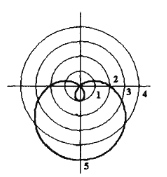
\includegraphics[width=0.4\textwidth]{2009A20.PNG}
    \end{center}

    \item %% Problem 84
    Pop Eye takes his family sailing. They leave dock A and sail 1.5 miles on a course of $30\degree$ to buoy B. They turn and travel 1.75 miles 
    on a bearing of $110\degree$ to buoy C. How far is it from buoy C to dock A? (nearest tenth)

    \item %% Problem 85
    Use the angle of rotation, $\theta$ (nearest degree), where $0\degree<\theta<90\degree$, to transform the conic $x^2+xy+y^2=3$ into an equation 
    that does not contain an $xy$ term. The equation is:

    \item %% Problem 86
    The circles $x^2+y^2+3x-6y+5=0$ and $2x^2+2y^2+5x-6y+3=0$ intersect in two points. The slope of the line through the two points of intersection is:
    
    \item %% Problem 87
    It is precisely 2:45 pm on a circular clock. What is the measure of the smaller angle formed by the minute hand and the hour hand of the clock?

    \item %% Problem 88
    $y^2-x^2=0$ is an equation of a degenerate conic. Which of the following is the best graphical representation of this equation?

    \item %% Problem 89
    Vector $v=(2,9)$ is perpendicular to vector $w=(4,k)$. Find $k$.

    \item %% Problem 90
    The graph shown is the graph of which of the following equations.
    \begin{center}
        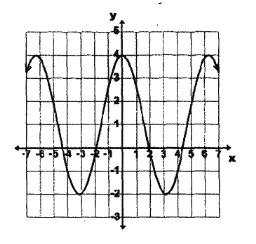
\includegraphics[width=0.4\textwidth]{2009A55.PNG}
    \end{center}

    \item %% Problem 91
    Point $P$ has polar coordinates of $(4,\frac{2\pi}{3})$ and rectangular coordinates of $(x,y)$. Where does point $P$ lie on the Cartesian coordinate plane?

    \item %% Problem 92
    Willie Dublett deposits \$500 in a bank account with an interest rate of 2.5\% compounded monthly.
    How many months will it take for his balance to reach \$750?

    \item %% Problem 93
    Determine the range of $f(x)=2+3\cos(4x-5)$.

    \item %% Problem 94
    A ramp is 18 ft. long and the angle of elevation of the ramp from the ground to the platform 
    is 15$\degree$ 10' 5''. Find the height of the platform. (nearest approximation)

    \item %% Problem 95
    The point $P(2,1)$ is rotated clockwise around the origin to point $(-1,-2)$. The angle of rotation, to the nearest degree, is:

    \item %% Problem 96
    The center of the circle, $x^2+y^2-4x-6y+9=0$, is \blank units from the origin. (nearest tenth)

    \item %% Problem 97
    A Ferris wheel has a radius of 7 meters and turns at 6 revolutions per minute. The bottom of the Ferris wheel is 1 meter above the ground.
    The height $h$ of a passenger above the ground varies sinusoidally with time $t$. Which of the following equations best describes the relationship between $h$ and $t$?
    
    \item %% Problem 98
    Which of the following is true about the relation $f(x)=x^2+2x+2$?
    
    \item %% Problem 99
    How many leafs are in the ``rose'' curve graph of the polar equation $r=3-4\sin(2\theta+5)$?

    \item %% Problem 100
    Which of the following is a reference angle for $1645\degree$?

    \item %% Problem 101
    If you start at $(-1.5,0)$ on the $x$-axis and travel horizontally 12 radians to the right, how many times will you cross the graph of $y=\sin(3x)$?

    \item %% Problem 102
    Tye Guhr drops a golf ball from a height of 10 feet. It bounces back to a height of 60\% of the distance it fell.
    How far has it traveled when it hits the ground the fourth time? (nearest inch)
    
    \item %% Problem 103
    Babe, Dizzy, and Yogi are playing ``toss and catch'' with a baseball. The bearing from Babe to Dizzy is 
    $254\degree$. The bearing from Yogi to Dizzy is 344$\degree$. The bearing from Yogi to Babe is $32\degree$. 
    The distance from Yogi to Dizzy is 20 feet. How far is it from Yogi to Babe? (nearest inch)

    \item %% Problem 104
    The equation $y=\blank$ will produce this graph.
    \begin{center}
        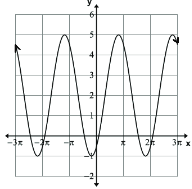
\includegraphics[width=0.3\textwidth]{2010A15.PNG}
    \end{center}

    \item %% Problem 105
    WHich of the following is a reference angle for $456\degree$?

    \item %% Problem 106
    Which of the following polar equations will produce this graph on a polar grid?
    \begin{center}
        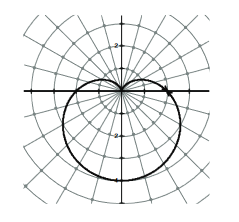
\includegraphics[width=0.3\textwidth]{2010A21.PNG}
    \end{center}

    \item %% Problem 107
    The graph of $4x^2+9y^2-16x+18y=2$ is a(n):

    \item %% Problem 108
    The eccentricity of the hyperbola $4x^2-y^2=4$ is:

    \item %% Problem 109
    If $\cos\theta < 0$ and $\tan\theta<0$ which quadrant will $\theta$ terminate in?

    \item %% Problem 110
    Let $||V_1||=15$ and $||V_2||=9$, where the direction angles of $V_1$ and $V_2$ are $20\degree$ and $80\degree$, respectively. Find $||V_1+V_2||$. (nearest tenth)

    \item %% Problem 111
    $\sin\theta \sec\theta + \cos\theta\csc\theta$ is equivalent to:

    \item %% Problem 112
    Willie Ketchit drops a golfball from a height of 10 meters. Each time it hits the ground it rebounds to a height of 50\% of the distance it fell.
    Find the total distance the golfball travels when it reaches the ground the third time. (nearest tenth)

    \item %% Problem 113
    The graph of $x^2-2xy+y^2+0x+0y+0=0$ is a \blank .

    \item %% Problem 114
    Which of the following is equivalent to $\frac{\sin\theta \tan\theta}{\sin(90\degree - \theta)}+\frac{\cot\theta}{\tan(90\degree-\theta)}$?

    \item %% Problem 115
    If $\cos x - \sin x = a$ and $\cos x + \sin x = b$, then $\cos^2 2x=$?

    \item %% Problem 116
    Let $||V_1||=9, ||V_2||=8$, where the direction angles of $V_1$ and $V_2$ are $60\degree$ and $150\degree$, respectively.
    Find the direction angle of $||V_1+V_2||$. (nearest degree)

    \item %% Problem 117
    The focus of the figure given by the equation $x^2+6x-12y+57=0$ is $(x,y)$. Find $x$.

    \item %% Problem 118
    Sir Vayor is trying to find the height of a flagpole. His eyes are 1.7 meters above the ground and he is standing 10 meters from the 
    base of the pole. The angle of elevation from his eyes to the top of the pole is 60$\degree$. Using this information, Sir Vayor computes the top of the flagpole to be: (nearest meter)

    \item %% Problem 119
    Using the equation $y=\frac{3}{4}\cos(2x-\frac{\pi}{3})-1$ which of the following has the largest numeric value?

    \item %% Problem 120
    The circles $(x-3)^2+(y+1)^2=16$ and $(x-4)^2+(y-2)^2=9$ intersect in two points. The slope of the line through the two points of intersection is:

    \item %% Problem 121
    Determine the range of $f(x)=2-4\cos(x+3)$.

    \item %% Problem 122
    $\frac{\sin\theta}{1+\cos\theta}+\frac{1+\cos\theta}{\sin\theta}$ is equivalent to:

    \item %% Problem 123
    Captain Ed Inberg went sailing on Lake Falcon. He sailed his scow from the dock 8 km on a bearing of $40\degree$. Then he changed course and sailed 5 km on a bearing of 
    $120\degree$. Then he decided to return to the dock. What bearing will Captain Ed have to sail to go straight back to the dock?

    \item %% Problem 124
    Given: $f(x)=2-4\sin(x+3)$. What quadrant(s) would the graph of $f(x)$ be in if the amplitude is cut in half, the vertical displacement is decreased by 5 and the phase shift is increased by 1?

    \item %% 125
    The Hole-In-One golf shop has periodic sales given by the function $G(m)=5+5\cos((\frac{\pi}{3})(m+3))$ where $m$ is the number of months 
    and $G(m)$ is the number of golf sets sold. If the store opened on Jan. 1, when did the maximum sales first occur?

    \item %% 126
    If you start at $\left(\frac{7\pi}{2},0\right)$ on the $x$-axis and travel horizontally 15.7 radians to the left, how many times will you cross 
    the graph of $y=2\sin(3x)$?

    \item % 127
    Given: $f(x)=3\cos[4\pi(x+1)]-2$. Find the sum of the numeric values of the period and the vertical displacement.

    \item % 128
    Meagan Money invested some money in the stock market. Her investment increased 8\% by the end of the first year,
    decreased 2\% by the end of the second year, and increased 12\% by the end of the third year. What was Meagan's average rate of 
    return over the three year period? (nearest tenth)

    \item % 129
    The vertex of a parabola is located at $(3,1)$ and the focus is located at $(3,3)$. Find the directrix of the parabola.

    \item % 130
    Given the function $f(x)=\sin x$, find the slope of the secant line between $x=0$ and $x=\frac{\pi}{2}$.

    \item %131
    Sir Benjamin Hall was looking at the circular face of the famous Big Ben clock. He noted that the time was 
    5:43 pm. What was the measure of the acute angle formed by the big hand and the little hand at that time?

    \item % 132
    Chip Shought hit his gold ball over a pond onto the edge of the green. He had to walk around the pond to his ball. He walked 70 yards on a bearing of 
    $250\degree$ from the tee. Then he walked 90 yards on a bearing of $50\degree$ to his ball. What was the straight line distance from the tee to his ball? (nearest yard)

    \item % 133
    I. C. Itt spotted a plane flying over his house. He noted that the angle of elevation from him to the plane was $32\degree 40'$ and he was 1,530 meters from his house.
    Using this information I. C. was able to determine the altitude of the plane. What was the altitude of the plane? (nearest meter)

    \item % 134
    If $x$ is in QIII then $\frac{1-\cos(2x)}{\sin(2x)} = \tan kx$ and $k$ equals: 

    \item % 135
    Given: $f(x)=3-2\sin(x+4)$, where the domain is ${x|x\in \text{ Reals}}$ and the range is 
    $\{f(x)|a\leq f(x)\leq b \text{ and } y\in \text{ Reals}\}$. Which of the following is not in the range?

    $\textbf{(A) } 1.5 \qquad \textbf{(B) } 3.124 \qquad \textbf{(C) } 2.04 \qquad \textbf{(D) } 5.333\dots \qquad \textbf{(E) }4.75$

    \item % 136
    The expression $(1-\cos\theta)(1+\cos\theta)(1+\cot^2\theta)$ is equivalent to:

    \item % 137
    $e^{3i}=\cos(3)+i\sin(3)$ is an example of \blank formula.

    \item % 138
    A circle with its center at the origin or the Cartesian x-y coordinate system has a radius of 3 units.
    If you start at $(-3,0)$ and travel on the circle $\frac{8\pi}{3}$ radians in a clockwise direction, where on the x-y coordinate plane will you stop at?

    \item % 139
    Sir Vayor used his theodolite to measure the height of the tower to be 17 ft 4'' tall. His theodolite was 5 ft from the level ground.
    What angle $x$ did he used to compute the height? (nearest second)
    \begin{center}
        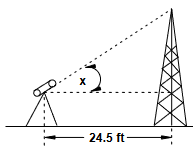
\includegraphics[width=0.3\textwidth]{2019A38.PNG}
    \end{center}

    \item % 140
    The graph of $f(x)$ shown below has a frequency of $0.6366197\dots$. Find $f(5.7)$. (nearest tenth)
    \begin{center}
        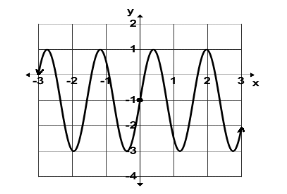
\includegraphics[width=0.3\textwidth]{2019A55.PNG}
    \end{center}

    \item % 141
    The center of a circle is in quadrant IV and the circumference of the circle is $16\pi$. The equation of the circle is 
    $x^2+y^2+ax+8y-39=0$. The value of $a$ is \blank.

    \item % 142
    If the distance from the point $(e,-12)$ to the line $y=\frac{3}{5}x+6$ is 
    $\frac{66}{\sqrt{34}}$, then $e=\blank$. ($e>-15$)

    \item % 143
    Consider the conic with equation $9x^2-4y^2-36x-24y-36=0$. If the coordinates of the foci are 
    $(a,b)$ and $(c,b)$ then $a+b+c=\blank$. (nearest tenth)

    \item % 144
    Two cables are attached to a vertical tower from a point on the ground. The angle between the cables is $20\degree$. The longer cable is 270 feet long and is 
    attached to the top of the tower. The shorter cable is attached to the tower 105 feet below the top of the tower. Find the length of the shorter cable. (nearest whole number)

    \item % 145
    Assume the temperature on a typical day in January in Idaho Falls varies sinusoidally with a low of 12$\degree$F at 5:00 AM and a high of 29$\degree$F at 5:00 PM. What is the expected temperature at midnight? (nearest tenth)

    \item % 146
    Angle $A$ is in quadrant II and angle $B$ is in quadrant III. If $\sin A = \frac{3}{5}$ and $\cos B = -\frac{5}{13}$, then $\tan(A+B)=\blank$. (nearest hundredth)

    \item % 147
    Find the angle between the vectors $u=\langle 4,-6\rangle$ and $v=\langle 12,8\rangle$ is \blank rad. (nearest hundredth)

    \item % 148
    Consider the sequence $1,5,12\frac{1}{2},20\frac{5}{6},26\frac{1}{24},\dots$. Find the eight term in the sequence (nearest hundredth)

    \item % 149
    A ball is dropped from a height of six feet and begins bouncing. Each bounce is three-fourths of the height of the previous bounce.
    Which bounce is the first bounce in which the height of the bounce is less than one foot?

    \item % 150
    Consider an ellipse in which the vertices are $(0,4)$ and $(10,4)$ and the endpoints of the minor axis are $(5,2)$ and $(5,6)$. What is the eccentricity of the ellipse? (nearest hundredth)

    \item % 151
    A boat is $2000$ km in front of you at an angle of $60\degree$ East of North. If you want to reach the boat in 4 hours, at what speed should you travel? (nearest tenth)

    \item % 152
    $y^2-x^2=0$ is an equation of a degenerate conic. Which of the following is the best graphical representation of this equation?

    \item % 153
    What is the wavelength of $y(x)=a+b\sin\left(\frac{n\pi x}{L}\right)$?

    \item % 154
    Where $V_1$ and $V_2$ are vectors in $\mathbb{R}^2$, if the norm of $V_1$ is 6, the norm of $V_2$ is 9, and the angle between them is 30,
    what is the norm of $V_1+V_2$? (nearest tenth)

    \item % 155
    Rachel accepted a job with a salary of \$95,000 the first year. During the next 19 years, she was given a 6\% raise each year. Find the total compensation she received over the 20-year period. (nearest dollar)

    \item % 156
    Given: $\sin(u)=-\frac{24}{25}$ and $\cos(v)=-\frac{3}{5}$. Both $u$ and $v$ are in quadrant III. Evaluate $\sec(u-v)$.

    \item % 157
    Audrey invested \$100,000 for 4 years. If the interest was compounded monthly rather than quarterly, she would have made \$345.93 more. What was the annual interest rate? (nearest hundredth)

    \item % 158
    Assume July temperatures vary sinusoidally in Denali National Park with a low of $48\degree$ at 4:00 AM and a high of $68\degree$ at 4:00 PM. The number $N$ of brown bears that are visible from Keith's campsite is given by $N(t)=(T-46\degree), 48\degree\leq T\leq 68\degree$, where $N(t)$ = the number of brown bears visible at time $t$ and $T$ is the temperature. How many brown bears are visible from Keith's campsite at 12:00 PM?

    \item % 159
    The circle $(x-6)^2+(y-12)^2=20$ is tangent to the circle $x^2+y^2=80$. The common internal tangent is a line with $x$-intercept $(a,0)$ and $y$-intercept $(0,b)$. $a+b=\blank$. (nearest whole number)

    \item % 160
    Justin obtained a sample of radioactive plutonium 234 at 5:00 AM on Wednesday. Only 1.510 g remained at 5:00 AM on Thursday and only 0.501 g remained at 7:00 PM on Thursday. Find the amount of plutonium Justin originally obtained. (nearest thousandth)
    

    For questions 161 and 162, consider the graph of a parabola with vertex $V(2,-6)$. Points $P(0,-4)$ and $Q(0,-8)$ both lie on the graph of the parabola.
    \item % 161
    The equation of the directrix of the graph of the parabola is $x=\blank$.

    \item % 162
    Point $T(a,0)$ lies on the graph of the parabola and point $F(e,f)$ is the focus of the graph of the parabola. $FT=\blank$. (nearest tenth)

    \item % 163
    Ship A leaves port at 1:00 PM and travels at an average speed of 18 mph on a bearing of $144\degree$. Ship B leaves port at 3:00 PM and travels at an average speed of 24 mph on a bearing of $284\degree$. At what time will the ships be 155 miles apart? (nearest minute)
    
    \item % 164
    Consider an ellipse such that for any point $P(e,f)$ that lies on the ellipse, the distance from $P$ to the point $(2,4)$ plus the distance from $P$ to the point $(14,4)$ equals 40. If the equation of the ellipse is $\frac{(x-h)^2}{a^2}+\frac{(y-k)^2}{b^2}=1$, then $b=\blank$. (nearest tenth)

    \item % 165
    The graph of $4x^2+5xy+2y^2-16=0$ is an ellipse in which the axes have been rotated $\blank\degree$. (nearest whole number)

    \item % 166
    The expression $(\sin\theta + \cos\theta)^2-1$ is equivalent to:

    \item % 167
    

\end{enumerate}

\section*{Solutions}
\begin{enumerate}[label=\bfseries\arabic*.]
    \item %% Problem 1
    6.3 units 

    \item %% Problem 2
    $-\frac{24}{25}$

    \item %% Problem 3
    2

    \item %% Problem 4
    9

    \item %% Problem 5
    217 ft 

    \item %% Problem 6
    $\sec\theta$

    \item %% Problem 7
    $x^2-y^2=2$

    \item %% Problem 8
    $6\frac{1}{4}$

    \item %% Problem 9
    0.66

    \item %% Problem 10
    $2\csc(x)$

    \item %% Problem 11
    76.0 s 
    
    \item %% Problem 12
    148

    \item %% Problem 13
    203 ft

    \item %% Problem 14
    cardioid

    \item %% Problem 15
    4

    \item %% Problem 16
    81

    \item %% Problem 17
    -3.4

    \item %% Problem 18
    294 rpm 

    \item %% Problem 19
    -5.00 

    \item %% Problem 20
    24i

    \item %% Problem 21
    1286

    \item %% Problem 22
    16 in 

    \item %% Problem 23
    21

    \item %% Problem 24
    6

    \item %% Problem 25
    D 

    \item %% Problem 26
    69.8$\degree$

    \item %% Problem 27
    cardioid 

    \item %% Problem 28
    24

    \item %% Problem 29
    523.6

    \item %% Problem 30
    11

    \item %% Problem 31
    D 

    \item %% Problem 32
    19.9 min 

    \item %% Problem 33
    -4

    \item %% Problem 34
    $-\frac{57}{8}$

    \item %% Problem 35
    4

    \item %% Problem 36
    1.8

    \item %% Problem 37
    68 ft 

    \item %% Problem 38
    40.6

    \item %% Problem 39
    33.66

    \item %% Problem 40
    153.9

    \item %% Problem 41
    1.07 ft 

    \item %% Problem 42
    11.1

    \item %% Problem 43
    $2\pi$

    \item %% Problem 44
    not a function 

    \item %% Problem 45
    62 ft
    
    \item %% Problem 46
    \$400

    \item %% Problem 47
    -34

    \item %% Problem 48
    175

    \item %% Problem 49
    556 mi 

    \item %% Problem 50
    75.4

    \item %% Problem 51
    8.9

    \item %% Problem 52
    39.75

    \item %% Problem 53
    1.2

    \item %% Problem 54
    $40\degree$

    \item %% Problem 55
    eccentricity

    \item %% Problem 56
    $69.8\degree$

    \item %% Problem 57
    $-3 \frac{3}{7}$

    \item %% Problem 58
    D 

    \item %% Problem 59
    $8+8i$

    \item %% Problem 60
    $1.2\degree$

    \item %% Problem 61
    $\frac{3}{4}$

    \item %% Problem 62
    -3.75

    \item %% Problem 63
    1

    \item %% Problem 64
    \$520.00

    \item %% Problem 65
    $5-2\sin\frac{1}{3}(-4x+5\pi)$

    \item %% Problem 66
    line
    
    \item %% Problem 67
    $8\pi$

    \item %% Problem 68
    1

    \item %% Problem 69
    2

    \item %% Problem 70
    15$\degree$

    \item %% Problem 71
    6

    \item %% Problem 72
    11' 2'' 

    \item %% Problem 73
    $x+2y=17$

    \item %% Problem 74
    $(\frac{8}{17},\frac{15}{17})$

    \item %% Problem 75
    $-\frac{1}{2}$

    \item %% Problem 76
    3.6 km

    \item %% Problem 77
    $2\sec(\frac{\pi}{2}x)$

    \item %% Problem 78
    directrix
    
    \item %% Problem 79
    16$\degree$ 41' 57''

    \item %% Problem 80
    $\frac{5\pi}{3}$

    \item %% Problem 81
    $\sin^2\theta$

    \item %% Problem 82
    $y=-1$

    \item %% Problem 83
    $r=2-3\sin\theta$

    \item %% Problem 84
    2.5 miles 

    \item %% Problem 85
    $3x^2+y^2=6$

    \item %% Problem 86
    $\frac{1}{6}$

    \item %% Problem 87
    $172.5\degree$

    \item %% Problem 88
    intersecting lines 

    \item %% Problem 89
    $-\frac{8}{9}$

    \item %% Problem 90
    $y=1+3\cos(x)$

    \item %% Problem 91
    QII 

    \item %% Problem 92
    195

    \item %% Problem 93
    $[-1,5]$

    \item %% Problem 94
    4' 8.52''

    \item %% Problem 95
    143$\degree$

    \item %% Problem 96
    3.6

    \item %% Problem 97
    $h=8-7\cos\left(\frac{\pi}{5}t\right)$

    \item %% Problem 98
    neither even nor odd function 

    \item %% Problem 99
    4

    \item %% Problem 100
    $25\degree$

    \item %% Problem 101
    11

    \item %% Problem 102
    33' 6'' 

    \item %% Problem 103
    29' 11''

    \item %% Problem 104
    $2+3\sin(x-1)$

    \item %% Problem 105
    $84\degree$

    \item %% Problem 106
    $r=2-2\sin\theta$

    \item %% Problem 107
    ellipse 

    \item %% Problem 108
    $\sqrt{5}$

    \item %% Problem 109
    QIII only 

    \item %% Problem 110
    21.0

    \item %% Problem 111
    $\frac{\sec^2\theta}{\tan\theta}$

    \item %% Problem 112
    25.0 m 

    \item %% Problem 113
    hyperbola 

    \item %% Problem 114
    $\sec^2 \theta$

    \item %% Problem 115
    $2ab$

    \item %% Problem 116
    $48\degree$

    \item %% Problem 117
    $(-3,4)$

    \item %% Problem 118
    13 m 

    \item %% Problem 119
    period 

    \item %% Problem 120
    $-\frac{1}{3}$

    \item %% Problem 121
    $[-2,6]$

    \item %% Problem 122
    $2\csc\theta$

    \item %% Problem 123
    $249\degree$

    \item %% Problem 124
    III \& IV

    \item %% Problem 125
    3 months 

    \item %% 126
    15

    \item % 127
    -1.5

    \item % 128
    5.8\%

    \item % 129
    $y=-1$

    \item % 130
    $\frac{2}{\pi}$

    \item % 131
    $86.5\degree$

    \item % 132
    34 yds 

    \item % 133
    981 meters 

    \item % 134
    1

    \item % 135
    D 

    \item % 136
    1 

    \item % 137
    Euler's 

    \item % 138
    Quadrant I 

    \item % 139
    26$\degree$ 43' 15''

    \item % 140
    -2.4

    \item % 141
    -6

    \item % 142
    -8

    \item % 143
    1.0

    \item % 144
    204 ft

    \item % 145
    18.3$\degree$F 

    \item % 146
    0.59

    \item % 147
    1.57

    \item % 148
    15.50

    \item % 149
    7

    \item % 150
    0.92

    \item % 151
    8.3 km/min 

    \item % 152
    intersecting lines 

    \item % 153
    $2L/n$

    \item % 154
    11.6

    \item % 155
    \$3,494,631

    \item % 156
    $\frac{125}{117}$

    \item % 157
    8.66\% 

    \item % 158
    17

    \item % 159
    30

    \item % 160
    10.008 g 

    \item % 161
    $\frac{5}{2}$

    \item % 162
    18.5

    \item % 163
    6:04 PM 

    \item % 164
    19.1

    \item % 165
    34

    \item % 166
    $\sin2\theta$

    \item % 167
    
\end{enumerate}

\end{document}